\documentclass[12pt]{article}
\usepackage[utf8]{inputenc}

\usepackage{enumerate}
\usepackage{listings}
\usepackage{pgfplots}
\usepackage{tikz}
\usepackage{svg}
\usepackage{graphicx}
\usepackage{setspace}
\usepackage{makecell}
\usepackage{caption}
\usepackage{subcaption}
\usepackage{pgf-umlsd}
\usepackage{epstopdf}
\usepackage{bytefield}
\usepackage{amsmath}
\usepackage{csquotes}
\usepackage[nottoc,numbib]{tocbibind}
\usepackage[section]{placeins}
\usepackage{tgtermes}
\usepackage{color}
\usepackage{hyperref}

\usetikzlibrary{shapes.geometric}
\usetikzlibrary{decorations.text}
\usetikzlibrary{positioning}
\usetikzlibrary{fit,shapes}

\hypersetup{
colorlinks,
citecolor=black,
filecolor=black,
linkcolor=black,
urlcolor=black
}

\lstloadlanguages{TeX}

\definecolor{lightred}{rgb}{1,0.7,0.71}

\begin{document}

    \thispagestyle{empty}
{\fontfamily{qtm}\selectfont
\begin{figure}[htbp]
    \centering
    
\includegraphics[scale=1.5]{img/agh-logo.pdf}
\end{figure}

\centerline{\small\textbf{AKADEMIA GÓRNICZO-HUTNICZA IM. STANISŁAWA STASZICA W KRAKOWIE}}
\vspace{1em}
\centerline{\small\textbf{WYDZIAŁ INFORMATYKI, ELEKTRONIKI I TELEKOMUNIKACJI}}
\vspace{1em}
\centerline{\small INSTYTUT Informatyki}
\vspace{2em}
\centerline{\Large Praca dyplomowa}
\vspace{2em}
\centerline{\textit{\large Validation of QUIC protocol usefullness in interactive communication}}
\vspace{1em}
\centerline{\textit{\large Ocena przydatności protokołu QUIC w komunikacji interaktywnej}}
\vspace{3em}

\begin{table}[h]
    \begin{tabular}{l l}
        Autor             & Michał Śledź              \\
        Kierunek studiów: & Informatyka               \\
        Opiekun pracy:    & dr inż.\ Łukasz Czekierda \\
    \end{tabular}
\end{table}

\null
\vfill
\centerline{Kraków, 2021}
}
    \clearpage

    \tableofcontents
    \clearpage
    \listoffigures
    \clearpage
    \listoftables
    \clearpage

    \section{Introduction}
\label{sec:introduction}

An interactive communication is bidirectional data exchange between people or people and machines.
It consists of two or more participants and has to be responsive meaning the result of performed action is delivered almost immediately.
In many cases interactive communication has to be also secure and reliable.
Examples of interactive communication are controlling remote robot in tele-surgery, doing exercises in tele-rehabilitation and
some types of multimedia sessions e.g.\ video conference, collaborative work or chat.
On the other hand to interactive communication does not belong exchanging emails (time between subsequent messages is too big) or
video on demand and streaming (they are not bidirectional).

Years of researches, protocol improvements and network devices optimizations have made interactive communication really fast.
We can talk with another person almost in the real time with a delay of several milliseconds.
Having said that it is perfectly correct to ask a question whether communication can be even faster, more effective and reliable and whether it is still worth to make improvements while we already have well prospering ecosystem.
In 2006 Prof.\ Edward Delp said:
\begin{displayquote}
    Is video coding dead?
    Some feel that, with the higher coding efficiency of the H.264/MPEG-4 Advanced Video Coding (AVC) standard (2x as compared to MPEG-2), perhaps there is not much more to do.
    I must admit that I have heard this \textquote{compression is dead} argument at least four times since I started working in image and video coding in 1976.\cite{4015574}
\end{displayquote}
Despite the fact that we are able to achieve very good performance in video conferencing systems there is still much to do.
Serious gaming, tele-surgery and tele-rehabilitation are all subject to tactile internet in which reliability, security and low latency are fundamental.
In such cases delay of 1 ms is desirable~\cite{the-tactile-internet}.

On the other hand, complexity of current standards makes them hard to implement, monitor and maintain.
One of them is WebRTC which uses over 10 different protocols and leaves implementation of signalling plane to the user.

QUIC is a new transport protocol standardized in RFC 9000 on May in 2021 and provides interesting and promising set of features.
%Its integration with TLS 1.3 significantly reduces connection establishment time while stream multiplexing in a single connection resolves head of line blocking problem of HTTP/2.
%QUIC introduces also special connection identifiers that prevents from additional handshakes in case of network switching and defines own flow control and congestion control mechanisms that are based on TCP ones.
%QUIC packets are encapsulated in UDP datagrams which makes QUIC user level protocol i.e.\ there is no need to modify kernel implementation to provide operating system with support for QUIC\@.
%
QUIC is mostly deployed in conjunction with a new version of HTTP called HTTP/3 and is intended to replace TCP and HTTP/2.
Therefore most publications are focused on web domain comparing QUIC and HTTP/3 with TCP/TLS and HTTP/2.

However, it turns out that a lot of QUIC features mainly stream multiplexing, pluggable congestion control, integration with TLS 1.3
or enhanced connection establishment mechanism can be useful in other domains.
As a result a number of IETF drafts emerged to expand QUIC to new areas.
The most important one is \textit{An Unreliable Datagram Extension to QUIC}.
It allows for combining reliable and unreliable data exchange in the same QUIC connection.

This document tries to answer a question whether QUIC can introduce significant improvement in terms of interactive communication.
To this end, analysis of QUIC encryption, loss detection and flow control mechanisms as well as number of tests and experiments have been performed.

The structure of this document is as follows.
Section~\ref{sec:state-of-the-art} presents state of the art and defines problems that will be addressed in this document.
Section~\ref{sec:quic-overview} introduces basic concepts of QUIC and compares QUIC to other transport protocols.
Section~\ref{sec:quic-in-webrtc} presents how QUIC can simplify WebRTC protocol stack.
It also describes packet encryption process in QUIC, answers the question if header encryption introduces significant overhead to the whole packet encryption and compares QUIC encryption process with RTP one.
Section~\ref{sec:datagrams} is dedicated to DATAGRAM frames in QUIC -- how they work and behave in different scenarios.
Section~\ref{sec:conclusions} concludes this document.

    \clearpage
    \section{State of the art}
\label{sec:state-of-the-art}

\textit{The QUIC Fix for Optimal Video Streaming} article~\cite{the-quic-fix-for-optimal-video-streaming} introduces unreliable data transmission over QUIC and presents how combination of reliable and unreliable transmission fares in video streaming and outperforms TCP and reliable mode of QUIC\@.
Authors of this document tag H.264 video frames depending on their importance.
\textit{I-Frames} which are independent frames meaning they can be displayed without any additional frames are marked to be sent reliably.
\textit{P-Frames} which are much smaller in size and code only the difference between \textit{I-Frame} and the next frame are marked to be sent unreliably.
The same approach is applied to \textit{B-Frames} that depends on both \textit{I-Frames} and \textit{P-frames}.
Authors state that the loss of \textit{P-Frames} or \textit{B-Frames} has minimal or no impact on the user's quality of experience (QoE).
They use i.a. \textit{buffering ratio (bufRatio)} and \textit{rate of buffering (rateBuf)} metrics to measure the difference in performance of streaming video over codec-agnostic DASH protocol used with TCP, traditional QUIC and QUIC with addition of unreliable transmission.
\textit{BufRatio} is the amount of time spent on buffering video comparing to the total session time (i.e.\ playing plus buffering time), represented as a percentage.
\textit{RateBuf} is the frequency of the buffering events~\cite{impact-of-video-quality-on-user-engagement}.
As a result, \textit{bufRatio}, with packet loss set to 0.64\%, for TCP is 105\%, for QUIC is 30\% and for QUIC with addition of unreliable data transmission is less than 1\%.
\textit{RateBuf}, with the same packet loss, is equal to 50\% for TCP, 19\% for QUIC and nearly 0\% for QUIC with addition of unreliable data transmission.

\textit{QUIC: Better for what and for whom?} article~\cite{quic-better-for-what-and-for-whom} compares the page load time (PLT) for HTTP/2 requests over QUIC and TCP/TLS in different network conditions and architectures as well as for different website complexities.
Authors prepared both local and remote testbeds.
In the remote one client's machine is connected to the Internet over ADSL (to router over Ethernet or Wi-Fi) or 4G\@.
Different network conditions mean different packet loss rate and delay.
In case of complexity of site there is Youtube service in which different resources might be distributed over many servers and Doctor (website of the ANR project) website where ale files are located on the same server.
Authors concludes that QUIC outperforms HTTP/2 over TCP/TLS in unstable networks but in case of stable and reliable networks the benefits of QUIC are not so obvious.

\textit{Game of protocols: Is QUIC ready for prime time streaming?} article~\cite{game-of-protocols} compares QUIC and TCP in HAS (HTTP adaptive streaming) applications.
To this end, authors performed experiments in four scenarios.
Frame-seek scenario is about seeking to the specified frame in the video.
Connection-switch scenario is about changing the connection from e.g.\ Wi-Fi to 3G\@.
Multiplexing scenario is about comparing different stream multiplexing techniques i.e.\ HTTP/1.1 over varying number of TCP connections, HTTP/2 with parallel requests over a single TCP connection and QUIC over a single UDP connection.
Fairness scenario is about checking fairness of congestion control mechanisms while there are multiple competing clients.
Authors also used three different adaptive algorithms: BASIC, SARA and BBA-2.
In the frame-seek scenario for BASIC algorithm QUIC behaved better by reducing bufRatio (called by authors rebuffer rate) from 3\% for WiFi and LTE to 1\% for WiFi and 2\% for LTE\@.
For 3G networks, QUIC reduced bufRatio from 5\% to 2\%.
For SARA and BBA-2 algorithms the results are also in favor of QUIC\@.
In the WiFi-LTE connection-switch scenario, QUIC reduced numerically bufRatio by 1\%, from 5\% to 4\% for BBA-2, from 4\% to 3\% for SARA and from 3\% to 2\% for BASIC\@.
Average playback bitrates also were a little higher for QUIC\@.
In the WiFi-3G connection-switch scenario, QUIC also behaved better and the reduction of bufRatio was similar except for BASIC algorithm where QUIC reduced bufRatio from 13\% to 6\%.
Evaluation of different multiplexing techniques showed that in the typical network conditions all three methods resulted in the similar average playback bitrate.
In the large delay and typical loss network, QUIC performed best.
For typical delay and large loss as well as for large delay and large loss, HTTP/1.1 with varying number of TCP connections was better than QUIC\@.
HTTP/2 over single TCP connection didn't manage to beat any of the other multiplexing techniques in any of the network conditions.
Fairness examination of congestion control mechanisms in TCP and QUIC showed that for typical packet loss and delay both protocols guarantee fair resource access for competing clients which results in the similar average playback bitrate.
In the large loss scenario single QUIC client was able to achieve higher bitrate (about 37\%) than single TCP client.
For competing clients, QUIC still was able to achieve better bitrate than TCP (about 40\%).
In the large delay scenario, the results were similar to the large loss scenario.
The last one scenario with large loss and large delay showed that TCP client was able to achieve higher bitrate (about 16\%) both when competing and not competing with QUIC client.

The objective of this document is to overview QUIC in terms of one more domain -- interactive communication.
The main question addressed here is which QUIC features can improve interactive communication.
By improvement I mean better adoption to changing network parameters and faster recovery after packet loss as well as reducing complexity of current systems and making them more developer friendly.

    \clearpage
    \section{QUIC overview}
\label{sec:quic-overview}
QUIC is a connection-based, multistream protocol that uses UDP under the hood. 
It is integrated with TLS and provides own congestion control and flow control mechanisms.
Data sent over QUIC is delivered in a reliable, ordered way.
Together with QUIC there comes a new version of HTTP called HTTP/3.

This section outlines main features of QUIC and compares QUIC to the other transport protocols.

\subsection{Packet types in QUIC}
\label{subsec:quic-packet-types}
The most outer entity in QUIC is a packet.
Each QUIC packet consists of a header that can take long or short form and one or more QUIC frames.
QUIC packets are directly encapsulated into UDP datagrams.
This is illustrated in figure~\ref{fig:quic-packet-format}.
A single UDP datagram can also coalesce many QUIC packets, however, this feature is not important in terms of regular data exchange.

\begin{figure}
    \centering
    \begin{bytefield}{32}
        \begin{leftwordgroup}{\tiny UDP header}
            \bitbox{16}{\tiny source port} & \bitbox{16}{\tiny destination port} \\
            \bitbox{16}{\tiny length} & \bitbox{16}{\tiny checksum}
        \end{leftwordgroup} \\
        \begin{leftwordgroup}{\tiny UDP data}
            \begin{rightwordgroup}{\tiny QUIC packet}
                \wordbox{1}{\tiny quic header} \\
                \wordbox[tlr]{1}{\tiny  quic frames} \\
                \wordbox[blr]{1}{\tiny $\cdots$}
            \end{rightwordgroup}
        \end{leftwordgroup}
    \end{bytefield}
    \caption{QUIC packet format}
    \label{fig:quic-packet-format}
\end{figure}

QUIC defines two types of header: short and long.
Figure~\ref{fig:short_header} illustrates Short Header form.
The first byte encodes miscellaneous flags.
Next, there is a destination connection ID that takes at most 20 bytes and a packet number that takes from 1 to 4 bytes.
Total size of Short Header is from 2 to 25 bytes.
Fields marked with red color are subject to an encryption process.
On the other hand Long Header additionally includes version, destination connection ID length, source connection ID length and source connection ID\@.
Flags differ a little comparing to the Short Header but together with a packet number length they also take 1 byte.

\begin{figure}[h]
    \centering
    \begin{bytefield}[bitwidth=4em]{8}
        \bitheader{0-7} \\
        \bitbox{1}{\tiny header form} & \bitbox{1}{\tiny fixed bit} & \bitbox{1}{\tiny spin bit} & \bitbox{2}[bgcolor=lightred]{\tiny reserved bits} & \bitbox{1}[bgcolor=lightred]{\tiny key phase} & \bitbox{2}[bgcolor=lightred]{\tiny packet number length} \\
        \wordbox{1}{\tiny destination connection ID (0 - 160)} \\
        \wordbox{1}[bgcolor=lightred]{\tiny packet number (8 - 32)}
    \end{bytefield}
    \caption{Short Header}
    \label{fig:short_header}
\end{figure}

QUIC introduces also different types of packets and frames.
Depending on specific packet type, it can contain different frame types.
For example \textit{Handshake} packet can contain \textit{CRYPTO}, \textit{PING}, \textit{PADDING}, \textit{ACK} or \textit{CONNECTION\_CLOSE} frames.
We can divide packet types basing on header form they use.
Following packet types use Long Header: \textit{Version Negotiation}, \textit{Initial}, \textit{0-RTT}, \textit{Handshake}, \textit{Retry}.
They are sent at the beginning of communication and therefore they are not covered more here.

Packet that uses Short Header is called \textit{1-RTT}.
1-RTT packets are sent after version and 1-RTT keys negotiation.
In an interactive communication they are main packets and they will, for example, convey media data.
1-RTT packet format is illustrated in figure~\ref{fig:1rtt-packet-format}.

\begin{figure}[h]
    \centering
    \begin{bytefield}[bitwidth=3.5em]{8}
        \bitheader{0-7} \\
        \begin{leftwordgroup}{\tiny short \\ \tiny header}
            \bitbox{1}{\tiny header form} & \bitbox{1}{\tiny fixed bit} & \bitbox{1}{\tiny spin bit} & \bitbox{2}[bgcolor=lightred]{\tiny reserved bits} & \bitbox{1}[bgcolor=lightred]{\tiny key phase} & \bitbox{2}[bgcolor=lightred]{\tiny packet number length} \\
            \wordbox{1}{\tiny destination connection ID (0 - 160)} \\
            \wordbox{1}[bgcolor=lightred]{\tiny packet number (8 - 32)}
        \end{leftwordgroup} \\
        \wordbox[tlr]{1}[bgcolor=lightred]{\tiny payload} \\
        \wordbox[blr]{1}[bgcolor=lightred]{\tiny $\cdots$}
    \end{bytefield}
    \caption{1-RTT packet format}
    \label{fig:1rtt-packet-format}
\end{figure}


\subsection{Security}
QUIC is integrated with TLS 1.3 providing confidentiality, integrity and authenticity of its packets.
Integration with TLS 1.3 is described in details in RFC 9001 \cite{rfc9001} and is based on negotiating both transport and cryptographic parameters in a single connection handshake.
This results in low-latency connection establishment (see section \ref{subsec:low-latency-conn-est}).
On the other hand there is no possibility to send unencrypted data over QUIC.

\subsection{Low-latency connection establishment}
\label{subsec:low-latency-conn-est}
Integration with TLS 1.3 results in reduction of handshakes needed for establishing a connection.
Unlike TCP, QUIC can perform both transport and cryptographic handshakes simultaneously by sending in its Initial packet data required by TLS.
This is presented in figure \ref{fig:low-latency-conn-est}.

\begin{figure}
    \centering
    \begin{subfigure}{.5\textwidth}
        \begin{sequencediagram}
            \newinst{client}{Client}
            \newinst[3]{server}{Server}
            \mess{client}{TCP SYN}{server}
            \mess{server}{TCP SYN + ACK}{client}
            \mess{client}{TCP ACK}{server}
            \postlevel
            \mess{client}{TLS ClientHello}{server}
            \mess{server}{TLS ServerHello}{client}
            \mess{client}{TLS Finished}{server}
            \postlevel
            \mess{client}{HTTP REQ}{server}
            \mess{server}{HTTP RES}{client}
        \end{sequencediagram}
        \caption{HTTP request in TCP}
        \label{subfig:http-req-tcp}
    \end{subfigure}%
    \begin{subfigure}{.5\textwidth}
        \begin{sequencediagram}
            \newinst{client}{Client}
            \newinst[3]{server}{Server}
            \mess{client}{QUIC}{server}
            \mess{server}{QUIC}{client}
            \mess{client}{QUIC}{server}
            \postlevel
            \mess{client}{HTTP REQ}{server}
            \mess{server}{HTTP RES}{client}
        \end{sequencediagram}
        \caption{HTTP request in QUIC}
        \label{subfig:http-req-quic}
    \end{subfigure}
    \caption{HTTP request comparison}
    \label{fig:low-latency-conn-est}
\end{figure}

Standard HTTP request using TCP/TLS stack requires 3-RTT (Round Trip Time).
Round Trip Time is a time needed for transporting a message from one side to the other and back again.
In TCP/TLS scenario, we need to perform separate handshakes for TCP and TLS which results in 2-RTT.
After this time we are able to send HTTP request which takes additional 1-RTT.
This scenario is presented in figure \ref{subfig:http-req-tcp}.

QUIC takes another approach.
It combines transport and cryptographic handshakes reducing time needed for establishing a connection.
In such a case sending HTTP request and receiving a response takes 2-RTT. 
This scenario is presented in figure \ref{subfig:http-req-quic}.

However, QUIC can reduce time needed for sending HTTP request and receiving a response even more.
In case when there was communication with the server previously and client cached information from it, it is possible to send HTTP request in the first round-trip of the connection.
This scenario is presented in figure \ref{fig:http-req-quic-0rtt}
\begin{figure}
\centering
    \begin{sequencediagram}
        \newinst{client}{Client}
        \newinst[3]{server}{Server}
        \mess{client}{QUIC}{server}
        \mess{client}{HTTP REQ}{server}
        \postlevel
        \mess{server}{QUIC}{client}
        \mess{server}{HTTP RES}{client}
        \postlevel
        \mess{client}{QUIC}{server}
    \end{sequencediagram}
\caption{HTTP request in QUIC with 0-RTT packets}
\label{fig:http-req-quic-0rtt}
\end{figure}


\subsection{Stream multiplexing}
QUIC is a multiplexed protocol which means we can open many streams in one QUIC connection.
Stream is an ordered sequence of bytes.
Each stream can be unidirectional or bidirectional and can be opened by a client or by a server.
Different types of streams can have different flow control limits (see section \ref{subsec:flow-control-and-congestion-control}).
Data in specific streams is carried independently which means that losing packet in one stream does not affect flow in other streams.
Figure \ref{fig:stream-multiplexing} shows this scenario.
One of the packets in stream 1 (marked as gray) was lost and needs to be retransmitted blocking subsequent packets (marked as black) on the receiver side.
They cannot be conveyed to the application layer until retransmission and reordering of the lost packet.
This is the source of so called head of line blocking problem which appears when we are trying to multiplex many HTTP requests in a single TCP connection.
Losing one packet stops the entire flow.
However, thanks to the stream multiplexing QUIC resolves this problem and streams 2 and 3 are not affected by the packet loss in stream 1.

\begin{figure}[h]
\centering
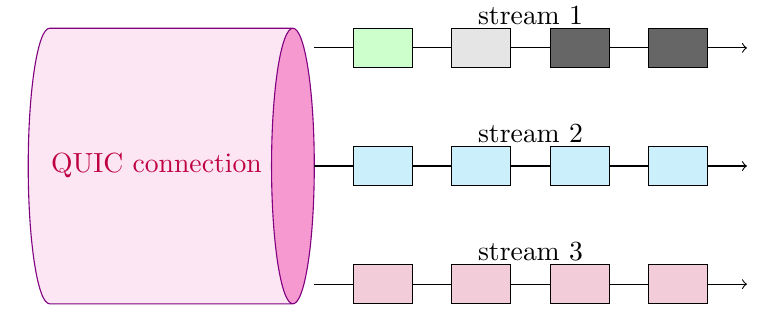
\begin{tikzpicture}

\node[cylinder, 
    draw = violet, 
    text = purple,
    style={transform shape},
    cylinder uses custom fill, 
    cylinder body fill = magenta!10, 
    cylinder end fill = magenta!40,
    minimum size = 3.5cm] (c) at (0,0) {QUIC connection};
    
\draw [->, postaction={decorate,decoration={raise=2ex, text along path,text align=center,text={stream 1}}}] (2, 1.5) -- (7.5, 1.5);
\filldraw [fill=green!20, draw=black] (2.5, 1.25) rectangle (3.25, 1.75);
\filldraw [fill=gray!20, draw=black] (3.75, 1.25) rectangle (4.5, 1.75);
\filldraw [fill=black!60, draw=black] (5, 1.25) rectangle (5.75, 1.75);
\filldraw [fill=black!60, draw=black] (6.25, 1.25) rectangle (7, 1.75);

\draw [->, postaction={decorate,decoration={raise=2ex, text along path,text align=center,text={stream 2}}}] (2, 0) -- (7.5, 0);
\filldraw [fill=cyan!20, draw=black] (2.5, -0.25) rectangle (3.25, 0.25);
\filldraw [fill=cyan!20, draw=black] (3.75, -0.25) rectangle (4.5, 0.25);
\filldraw [fill=cyan!20, draw=black] (5, -0.25) rectangle (5.75, 0.25);
\filldraw [fill=cyan!20, draw=black] (6.25, -0.25) rectangle (7, 0.25);

\draw [->, postaction={decorate,decoration={raise=2ex, text along path,text align=center,text={stream 3}}}] (2, -1.5) -- (7.5, -1.5);
\filldraw [fill=purple!20, draw=black] (2.5, -1.75) rectangle (3.25, -1.25);
\filldraw [fill=purple!20, draw=black] (3.75, -1.75) rectangle (4.5, -1.25);
\filldraw [fill=purple!20, draw=black] (5, -1.75) rectangle (5.75, -1.25);
\filldraw [fill=purple!20, draw=black] (6.25, -1.75) rectangle (7, -1.25);


\end{tikzpicture}
\caption{Stream multiplexing in a single QUIC connection}
\label{fig:stream-multiplexing}
\end{figure}

\subsection{Connection migration}
Each QUIC connection has a set of connection identifiers each of which can identify the connection.
Connection IDs can be variable length.
QUIC uses connection IDs to route packets to proper endpoint.
This way, as long as there is an alternative network path, QUIC is resilient to network changes avoiding restarting the connection when an endpoint changes its transport address (IP or port).

\subsection{Flow control and congestion control mechanisms}
\label{subsec:flow-control-and-congestion-control}

\subsection{Reliability}
QUIC is a reliable protocol which means it guarantees delivery of each packet sent by the endpoint.
Packets are delivered to the receiver side in the order they were sent.
However, there are different IETF drafts that expand QUIC with new features.
One of them called "An Unreliable Datagram Extension to QUIC"\cite{bider-ssh-quic-09} allows for sending unreliable messages over QUIC.
This can take place in simultaneously to the reliable communication.
Unreliable messages are not subject to flow control mechanisms however, they are congestion controlled.
Each unreliable message is also acknowledged so that application layer can be provided with the packet loss information.
Section \ref{sec:datagrams} describes Datagram extension in details.

\subsection{QUIC against other transport protocols}
\label{sec:quic_against_other_transport_protocols}
This section compares QUIC with three main transport protocols -- TCP, UDP and SCTP.  
\subsubsection{TCP}
Transmission Control Protocol -- connection based, stream oriented and reliable transport protocol.
It guarantees the order of messages and provides flow control and congestion control mechanisms.
One of the drawbacks of TCP is its head of line blocking problem.
If one TCP segment gets lost then all subsequent TCP segments that arrived to the recipient have to be buffered until retransmission of the lost segment.
When the lost segment finally arrives, buffered segments and retranssmited segment are arranged in the proper order and made available to the user who can read them from internal socket buffer.
This is the reason why HTTP/2 only partially solves head of line blocking problem of HTTP/1 -- there is still the same problem on TCP level.
\subsubsection{UDP}
User Datagram Protocol -- connection less, unreliable transport protocol. 
It does not preserve the order of messages. 
Datagrams, in this protocol, are not acknowledged nor congestion controlled.
It does not also introduce any flow control mechanisms.
Thanks to its simplicity and low bandwidth affection it is the base for RTP protocol which is widely used for transmitting multimedia.
Unlike TCP, UDP also allows for multicast transmission.
However, multicast is rarely used, mostly in local networks.
\subsubsection{SCTP}
Stream Control Transmission Protocol -- reliable, based on UDP, message oriented transport protocol.
Unlike TCP, SCTP is multi-stream protocol which means that it is not affected by head of line blocking problem. 
SCTP is partially ordered but it also allows for sending unordered messages. 
Another feature of SCTP is multi-homing in which an endpoint uses two different addresses. 
This introduces some kind of fault tolerance -- one address is designated as a primary and the other one can be used in case of failure of the first one.
Unfortunately SCTP is not widely used.
Its main domain is telecommunication as a lot of home routers does not handle SCTP properly.

\subsubsection{Summary}
Table \ref{tab:protocols_comparision} presents a short summary of transport protocols comparison.
\begin{table}[h]
\centering
\begin{tabular}{|c | c | c | c | c |} 
    \hline
    & TCP & UDP & SCTP & QUIC \\  
    \hline
    reliability & reliable & unreliable & reliable & reliable \\
    \hline
    transmission & byte oriented & message oriented & message oriented & byte oriented \\
    \hline
    flow control & yes & no & yes & yes \\
    \hline
    congestion control & yes & no & yes & yes \\
    \hline
    packets order & ordered & unordered & partially ordered & ordered \\
    \hline
    multistream & no & no & yes & yes \\
    \hline
\end{tabular}
\caption{\label{tab:protocols_comparision}Transport protocols comparison.}
\end{table}

    \clearpage
    %! suppress = EscapeAmpersand
\section{QUIC in WebRTC}
\label{sec:quic-in-webrtc}
This section outlines how QUIC can be used in WebRTC standard.

\subsection{WebRTC overview}
\label{subsec:webrtc-overview}
WebRTC is a standard that enables peer to peer (P2P) multimedia connections in web browsers when both peers are behind NATs without using any plugins.
It is natively implemented by all major browsers.
In WebRTC there are two planes -- media plane and signaling plane.
The former is responsible for relaying both media data (audio, video) and non-media data (chat messages, uploading and downloading files, etc.).
The later is responsible for negotiating session parameters like audio and video codecs or transport addresses.
The whole protocol stack is presented in figure~\ref{fig:webrtc-stack}.

\begin{figure}
    \centering
    \tikzstyle{rect}=[rectangle,minimum width=6cm,minimum height=1cm,draw=black,outer sep=0pt]
    \tikzstyle{base rect}=[rect,minimum width=12cm,outer sep=0pt]
    \tikzstyle{text rect}=[rectangle,minimum width=6cm,align=center,outer sep=0pt]
    \tikzstyle{multipart rect}=[rectangle split,rectangle split horizontal,rectangle split parts = 2,inner xsep = 0.0mm,outer sep=0pt,
    draw=black,align=center,minimum width=6cm,minimum height=1cm]
    \begin{tikzpicture}
        % ip
        \node (IP) [base rect,fill=gray!20] {IP};

        % media plane
        \node (UDP) [rect,fill=blue!20,above left=0.0cm of IP.north] {UDP};
        \node (ICE) [rect,fill=purple!20,above=0.0cm of UDP]  {ICE, STUN, TURN} ;
        \node (DTLS) [rect,fill=orange!20,above=0.0cm of ICE] {DTLS} ;
        \node (SRTP) [multipart rect,rectangle split part fill={green!20,yellow!20},above=0.0cm of DTLS] {\nodepart[text width=3cm]{one} SRTP \nodepart[text width=3cm]{two} SCTP} ;
        \node [text rect,above=0.0cm of SRTP]{Media Plane};

        % signaling plane
        \node (TCP) [rect,fill=blue!20,above right=0.0cm of IP.north]{TCP};
        \node (TLS) [rect,fill=purple!20,above=0.0cm of TCP] {TLS};
        \node (HTTP) [rect,fill=orange!20,above=0.0cm of TLS] {HTTP};
        \node (WS) [rect,fill=green!20,above=0.0cm of HTTP] {WS/Other};
        \node (SDP) [multipart rect,above=0.0cm of WS,rectangle split part fill={gray!20,yellow!20}] {\nodepart[text width=3cm]{one} SDP \nodepart[text width=3cm]{two} SIP/XMPP/\\Other};
        \node [text rect,above=0.0cm of SDP]{Signaling Plane};
    \end{tikzpicture}
    \caption{WebRTC protocol stack.}
    \label{fig:webrtc-stack}
\end{figure}

\subsubsection{Media plane}
\label{subsubsec:media-plane}
In media plane, media data is carried using RTP protocol which stands for Real-time Transport Protocol.
RTP protocol provides media packets with information that is not present in headers of UDP datagrams but is important in terms of multimedia transmission.
This information includes timestamps -- to know when data should be passed to video or audio decoder, sequence numbers -- to perform packets reordering, payload type -- to know which codec is used.
RTP packets are encrypted using cryptographic context negotiated during DTLS handshake.
DTLS handshake provides so called keying material which is used by both sides for creating actual keys used for protecting and unprotecting RTP packets.
Thanks to this we can encrypt only RTP payload (without header) and encapsulate whole RTP packet directly into UDP datagram omitting DTLS record layer.
Key derivation process as well as encryption and decryption mechanisms are described in SRTP (Secure Real-time Transport Protocol) which is a profile of RTP protocol.

On the other hand, non-media data is carried by SCTP\@.
Unlike RTP packets, SCTP datagrams are encapsulated in DTLS datagrams.

Besides SRTP and SCTP protocols there are ICE, STUN and TURN\@.
They are used for establishing a connection between peers even when both of them are behind NATs.

At the end, in most cases everything is carried in UDP datagrams.
However, in some specific scenarios (e.g.\ when some network blocks UDP traffic or allows only for traffic on port 443) TCP or TLS over TCP has to be used.

\subsubsection{Signaling plane}
Main protocol used in signaling plane is Session Description Protocol (SDP).
It defines format of messages that carry information about number of media tracks, their codecs, relationships between them, etc.
WebRTC does not define how to exchange these messages between peers.
Instead, it is user (i.e.\ someone using WebRTC API) responsibility.
In many cases it is done using a separate connection over WebSocket (WS) to a dedicated signaling server.
Figure~\ref{fig:webrtc-architecture} presents WebRTC architecture.

\begin{figure}
    \centering
    \begin{tikzpicture}[node distance = 4cm]
        \node (signaling server)[label=below:{Signaling server}] {
\includegraphics{cisco_icons/fileserver.eps}};

        \node (pc a) [below left=of signaling server,label=below:{PC A}] {
\includegraphics{cisco_icons/workstation.eps}}
        edge [<->, bend left=45] node[align=center,left] {signaling\\messages} (signaling server);
        \node (pc a firewall) [right=0.0cm of pc a,label=below:{NAT}] {
\includegraphics{cisco_icons/firewall.eps}};

        \node (pc b) [below right=of signaling server,label=below:{PC B}] {
\includegraphics{cisco_icons/workstation.eps}}
        edge [<->, bend right=45] node[align=center,right] {signaling\\messages} (signaling server);
        \node (pc b firewall) [left=0.0cm of pc b,label=below:{NAT}] {
\includegraphics{cisco_icons/firewall.eps}}
        edge [<->] node[above] {audio/video/non-media data} (pc a firewall);

    \end{tikzpicture}
    \caption{WebRTC architecture in P2P scenario}
    \label{fig:webrtc-architecture}
\end{figure}

\subsubsection{Why media plane uses SRTP instead of plain DTLS records}
As stated in section~\ref{subsubsec:media-plane}, RTP packets does not use DTLS record layer.
There are two reasons why.
First of all SRTP protects only RTP payload.
Encapsulating RTP packet in DTLS record would encrypt also RTP header.
The second reason is duplication of data.
Figure~\ref{fig:srtp-packet} illustrates format of an SRTP packet.
Fields that are specific to SRTP profile are \textit{SRTP MKI (Master Key Identifier)} and \textit{authentication tag}.
The rest of fields comes from usual RTP packet.
On the other hand figure~\ref{fig:dtls-packet} presents DTLS record.
We can see that DTLS record includes \textit{sequence number} field that is already in RTP header (they differ only in size) and some other fields like \textit{protocol version} or \textit{epoch}.
Total length of DTLS record header is equal to 104 bits (13 bytes).
All of this data is redundant in terms of multimedia communication.

\begin{figure}
    \centering
    \begin{bytefield}[bitwidth=0.8em]{32}
        \bitheader{0-31} \\
        \begin{rightwordgroup}{\tiny Authenticated \\ \tiny Portion}
            \bitbox{2}{\tiny V=2} & \bitbox{1}{\tiny P} & \bitbox{1}{\tiny X}
            & \bitbox{4}{\tiny CC} & \bitbox{1}{\tiny M} & \bitbox{7}{\tiny PT}
            & \bitbox{16}{\tiny sequence number} \\
            \bitbox{32}{\tiny timestamp} \\
            \bitbox{32}{\tiny synchronization source (SSRC) identifier} \\
            \begin{leftwordgroup}{\tiny 0 to 15 \\ \tiny items}
                \wordbox[tlr]{1}{\tiny contributing source (CSRC) identifiers} \\
                \wordbox[blr]{1}{\tiny $\cdots$}
            \end{leftwordgroup} \\
            \begin{leftwordgroup}{\tiny Optional \\ \tiny RTP \\ \tiny extensions}
                \bitbox{16}{\tiny defined by profile} & \bitbox{16}{\tiny length} \\
                \wordbox[tlr]{1}{\tiny header extension} \\
                \wordbox[blr]{1}{\tiny $\cdots$}
            \end{leftwordgroup} \\
            \begin{leftwordgroup}{\tiny Encrypted \\ \tiny Portion}
                \wordbox[tlr]{2}{\tiny payload} \\
                \bitbox[blr]{16}{} & \bitbox{8}{\tiny RTP padding} & \bitbox{8}{\tiny RTP pad count}
            \end{leftwordgroup}
        \end{rightwordgroup} \\
        \wordbox{1}{\tiny SRTP MKI (OPTIONAL)} \\
        \wordbox{1}{\tiny authentication tag (RECOMMENDED)}
    \end{bytefield}
    \caption{SRTP packet format}
    \label{fig:srtp-packet}
\end{figure}

\begin{figure}
    \centering
    \begin{bytefield}{32}
        \bitheader{0-31} \\
        \bitbox{8}{\tiny type} & \bitbox{16}{\tiny version} & \bitbox{8}{\tiny epoch} \\
        \bitbox{8}{\tiny epoch} & \bitbox{24}{\tiny sequence number} \\
        \bitbox{24}{\tiny sequence number} & \bitbox{8}{\tiny length} \\
        \bitbox{8}{\tiny length} & \bitbox{24}{\tiny fragment} \\
        \wordbox{1}{\tiny fragment}
    \end{bytefield}
    \caption{DTLS packet format}
    \label{fig:dtls-packet}
\end{figure}

\subsection{RTP encapsulation in QUIC}
\label{subsec:rtp-encapsulation-in-quic}
RTP packets should be sent unreliably therefore they must be encapsulated into DATAGRAM frames described in section~\ref{sec:datagrams}.
RTP over QUIC~\cite{engelbart-rtp-over-quic-00} proposes encapsulation presented in figure~\ref{fig:rtp-encapsulation-into-quic-packet}.

\begin{figure}
    \centering
    \begin{bytefield}[bitwidth=3.5em]{8}
        \wordbox{1}{\tiny short header} \\
        \begin{leftwordgroup}{\tiny DATAGRAM \\ \tiny frame}
            \wordbox{1}{\tiny length(i) (OPTIONAL)} \\
            \wordbox{1}{\tiny flow identifier(j)} \\
            \wordbox{1}{\tiny RTP packet}
        \end{leftwordgroup}
    \end{bytefield}
    \caption{RTP encapsulation into QUIC packet}
    \label{fig:rtp-encapsulation-into-quic-packet}
\end{figure}

There are two drawbacks of proposed solution.
The first one is duplication of data as \textit{sequence\_number} field is present both in a QUIC and RTP headers.
The second one is that RTP header will be entirely encrypted as a part of QUIC packet payload.
These caveats are the same as in the case of using DTLS instead of SRTP however, encapsulating RTP in QUIC will result in a much simpler protocol stack.
Comparison of WebRTC protocol stacks is presented in figure ~\ref{fig:webrtc-stack-comparision}

\begin{figure}
    \centering
    \tikzstyle{rect}=[rectangle,minimum width=6cm,minimum height=1cm,draw=black,outer sep=0pt]
    \tikzstyle{text rect}=[rectangle,minimum width=6cm,align=center,outer sep=0pt]
    \tikzstyle{multipart rect}=[rectangle split,rectangle split horizontal,rectangle split parts = 2,inner xsep = 0.0mm,outer sep=0pt,
    draw=black,align=center,minimum width=6cm,minimum height=1cm]
    \begin{subfigure}[b]{0.4\textwidth}
        \begin{tikzpicture}
            % ip
            \node (IP) [rect,fill=gray!20] {IP};

            % media plane
            \node (UDP) [rect,fill=blue!20,above=0.0cm of IP] {UDP};
            \node (ICE) [rect,fill=purple!20,above=0.0cm of UDP]  {ICE, STUN, TURN} ;
            \node (DTLS) [rect,fill=orange!20,above=0.0cm of ICE] {DTLS} ;
            \node (SRTP) [multipart rect,rectangle split part fill={green!20,yellow!20},above=0.0cm of DTLS] {\nodepart[text width=3cm]{one} SRTP \nodepart[text width=3cm]{two} SCTP} ;
        \end{tikzpicture}
        \caption{WebRTC stack.}
        \label{fig:webrtc-stack-comparision-standard}
    \end{subfigure}
    \hfill
    \begin{subfigure}[b]{0.4\textwidth}
        \begin{tikzpicture}
            % ip
            \node (IP) [rect,fill=gray!20] {IP};

            % media plane
            \node (UDP) [rect,fill=blue!20,above=0.0cm of IP] {UDP};
            \node (ICE) [rect,fill=purple!20,above=0.0cm of UDP]  {ICE, STUN, TURN} ;
            \node (QUIC) [rect,fill=orange!20,above=0.0cm of ICE] {QUIC} ;
            \node (RTP) [rect,fill=green!20,above=0.0cm of QUIC] {RTP} ;
        \end{tikzpicture}
        \caption{WebRTC stack with QUIC.}
        \label{fig:webrtc-stack-comparision-quic}
    \end{subfigure}
    \caption{Comparison of current WebRTC stack and alternative WebRTC stack when using QUIC protocol.}
    \label{fig:webrtc-stack-comparision}
\end{figure}

\subsection{QUIC packet encryption}
\label{subsec:packet-encryption}
This section outlines encryption process of QUIC packet.
In QUIC not only packet payload is encrypted but also some fields in packet header.

\subsubsection{Payload encryption}
Payload is encrypted using AEAD algorithm.
All cipher-suites used in TLS 1.3 are allowed in QUIC except \textit{AES\_128\_CCM\_8}.
Therefore we have \textit{AES\_128\_GCM}, \textit{AES\_256\_GCM}, \textit{CHACHA20\_POLY1305} and \textit{AES\_128\_CCM}.
Figure~\ref{fig:payload_enc} shows the process of payload encryption.
As a plain text we pass payload and as an associated data we pass plain header.
As a result we get a ciphertext and an authentication tag.

\begin{figure}[h]
    \centering
    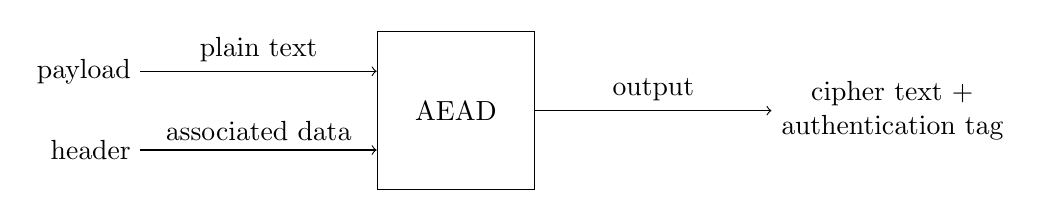
\begin{tikzpicture}
        \node (aead) [rectangle, draw=black, minimum width=2cm,minimum height=2cm] {AEAD};
        \node (aead in 0) [rectangle, minimum width=1cm,minimum height=1cm, above left=of aead.south east] {};
        \node (aead in 1) [rectangle, minimum width=1cm,minimum height=1cm, below left=of aead.north east] {};
        \node (payload) [left=3cm of aead in 0] {payload}
        edge [->] node[align=center,above] {plain text} (aead in 0);
        \node (header) [left=3cm of aead in 1] {header}
        edge [->] node[align=center,above] {associated data} (aead in 1);
        \node (cipher text) [align=center, right=3cm of aead] {cipher text + \\ authentication tag}
        edge [<-] node[align=center, above] {output} (aead);
    \end{tikzpicture}
    \caption{QUIC payload encryption scheme}
    \label{fig:payload_enc}
\end{figure}

\subsubsection{Header encryption}
Figure~\ref{fig:header_enc} shows the process of header encryption.
The first step is to get \textit{sample} from encrypted payload.
In most cases a sample is 16 bytes long and it is taken starting from $4 - pn\_len$ byte of encrypted payload.
In the next step the sample is encrypted and its first 5 bytes are taken as mask.
At the end we perform XOR operation on predefined header fields and mask.
As a result we get header with some fields being encrypted.
Algorithm used to encrypt sample depends on negotiated cipher-suite.
For example, if payload is encrypted with AES\_128\_GCM then sample will be encrypted using AES\_128\_ECB\@.

\begin{figure}[h]
    \centering
    \tikzset{XOR/.style={draw,circle, minimum width=1cm, minimum height=1cm, append after command={
    [shorten >=\pgflinewidth, shorten <=\pgflinewidth,]
    (\tikzlastnode.north) edge (\tikzlastnode.south)
    (\tikzlastnode.east) edge (\tikzlastnode.west)}}}
    \begin{tikzpicture}
        \node (xor) [XOR, scale=1.2] {};
        \node (encrypted header) [right=of xor] {encrypted header}
        edge [<-] node[align=center,above] {} (xor);
        \node (mask) [below left=of xor] {mask}
        edge [->, to path={-| (\tikztotarget)}] (xor.south);
        \node (sample) [left=of mask] {sample}
        edge [->] (mask);
        \node (payload) [left=of sample] {payload}
        edge [->] (sample);
        \node (header)  at (payload |- xor) {header}
        edge [->] (xor);
    \end{tikzpicture}
    \caption{QUIC header encryption scheme}
    \label{fig:header_enc}
\end{figure}

\subsection{Tests}
\label{subsec:tests}
Following tests are split into two scenarios.

In the first one I am comparing time needed for encrypting constant length QUIC header (22 bytes) and variable length QUIC payload.
QUIC payload encapsulates RTP packet.
Therefore it consists of constant length flow identifier (1 byte), constant length RTP header (12 bytes) and variable length RTP payload (from 100 to 1200 bytes).

In the second scenario I am comparing time needed for encrypting standalone variable length RTP payload (from 100 to 1200 bytes) and whole QUIC packet which consists of constant length QUIC header (22 bytes) and variable length QUIC payload.
QUIC payload has the same format as in the first test scenario.
Whole QUIC packet size can be obtained from the equation~\ref{eq:quic-packet-size}.
\begin{align}
    \begin{split}
        QUIC\_packet\_size & = RTP\_payload\_size + RTP\_header\_size \\
        & \quad + tag\_identifier + QUIC\_header\_size \\
        & = RTP\_payload\_size + 12 + 1 + 22 \\
        & = RTP\_payload\_size + 35
    \end{split}
    \label{eq:quic-packet-size}
\end{align}

In both test scenarios, encryption process was performed concurrently.

\subsubsection{Environment}
Test environment:
\begin{itemize}
    \item processor: Intel(R) Core(TM) i5-9600K CPU @ 3.70GHz, 6 Cores, 9 MB Cache
    \item memory: 16 GB RAM
    \item operating system: Linux
    \item library: ring 0.16.20
    \item language: Rust
    \item cipher-suite: AES\_128\_GCM
\end{itemize}

\subsubsection{Methodology}
For each RTP payload size following steps were performed:
\begin{itemize}
    \item collect 100 samples
    \item detect and remove outliers
    \item count average from remaining samples
\end{itemize}

\subsubsection{Results}
Figure~\ref{fig:header-payload-enc} presents time comparison between header and payload encryption process.
We can see that QUIC payload encryption time is between 220 and 450 ns.
For 400, 800 and 1200 RTP payload sizes we can observe shorter encryption time than for previous sizes.
This is probably because of concurrent execution of encryption process.
The data can be split across threads in a manner that allocates additional thread for 400, 800 and 1200 bytes.

\begin{figure}[h]
    \centering
    \begin{tikzpicture}
        \begin{axis}[xlabel={RTP payload size (bytes)},
        ylabel={Average time (ns)},
        legend style={legend pos=outer north east}]
            \addplot table[x=size,y=time] {data/quic-header-enc.table};
            \addlegendentry{Header encryption time}
            \addplot table[x=size,y=time] {data/quic-payload-enc.table};
            \addlegendentry{Payload encryption time}
        \end{axis}
    \end{tikzpicture}
    \caption{QUIC header vs QUIC payload encryption time}
    \label{fig:header-payload-enc}
\end{figure}

Figure~\ref{fig:rtp-payload-quic-packet-enc} presents time comparison between RTP payload and QUIC packet (with RTP packet inside) encryption process.
As in the first test scenario, for 400, 800 and 1200 RTP payload sizes we can observe shorter encryption time than for previous sizes.
Encryption of QUIC packet that encapsulates RTP packet is slower by 30--50ns comparing to standalone RTP payload encryption.
This is illustrated in figure~\ref{fig:rtp-payload-quic-packet-enc}.

\begin{figure}[h]
    \centering
    \begin{tikzpicture}
        \begin{axis}[xlabel={RTP payload size (bytes)},
        ylabel={Average time (ns)},
        legend style={legend pos=outer north east}]
            \addplot table[x=size,y=time] {data/quic-packet-enc.table};
            \addlegendentry{QUIC packet encryption time}
            \addplot table[x=size,y=time] {data/rtp-payload-enc.table};
            \addlegendentry{RTP payload encryption time}
        \end{axis}
    \end{tikzpicture}
    \caption{RTP payload vs QUIC packet (with RTP packet inside) encryption time}
    \label{fig:rtp-payload-quic-packet-enc}
\end{figure}

In summary, QUIC header encryption does not introduce a significant overhead for the entire QUIC packet encryption process.
Also, encryption of encapsulated RTP packet into QUIC packet is insignificantly slower than encryption of standalone RTP payload.

%\subsection{SSH}
%Secure Shell protocol allows for secure connections to remote machines over insecure network.
%It defines channels where each channel can be terminal session, forwarded connections etc. \cite{rfc4254}.
%Channels are flow controlled.
%One SSH connection can multiplex multiple SSH channels.
%SSH uses TCP under the hood which is also flow controlled.
%Figure \ref{fig:ssh-connection} presents architecture of SSH connection.
%
%\begin{figure}[h]
%    \begin{subfigure}[b]{0.4\textwidth}
%        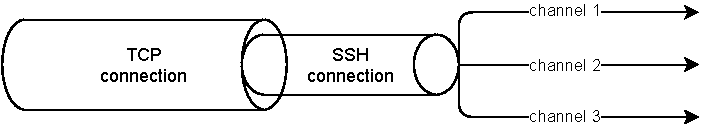
\includegraphics[width=\textwidth]{img/__06__current_standards_and_protocols/ssh.pdf}
%        \caption{SSH connection architecture.}
%        \label{fig:ssh-connection}
%    \end{subfigure}
%    \hfill
%    \begin{subfigure}[b]{0.4\textwidth}
%        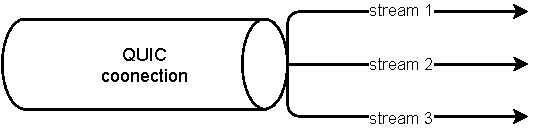
\includegraphics[width=\textwidth]{img/__06__current_standards_and_protocols/quic_ssh.pdf}
%        \caption{Alternative SSH connection architecture with QUIC protocol.}
%        \label{fig:quic-ssh-connection}
%    \end{subfigure}
%    \caption{Comparison of current SSH connection architecture and alternative SSH connection architecture using QUIC protocol.}
%\end{figure}
%
%According to \cite{bider-ssh-quic-09}, using QUIC connection we could remove one level of flow control, reduce connection handshakes from two (one for TCP and one for SSH) to one (only for QUIC) and use streams as SSH channels.
%This approach is presented on figure \ref{fig:quic-ssh-connection}.

    \clearpage
    \section{An Unreliable Datagram Extension to QUIC}
\label{sec:datagrams}
QUIC is by default a reliable protocol.
However there are plenty of situations where transmission speed is more important than reliability, especially in real-time communication.
\textit{An Unreliable Datagram Extension to QUIC} \cite{ietf-quic-datagram-02} introduces a new QUIC frame called DATAGRAM which carry data unreliably.

According to \cite{ietf-quic-datagram-02} DATAGRAM frames are not retransmitted.
They are sent alongside the STREAM frames so they use the same cryptography context but they don't affect flow-control limits.
Each DATAGRAM frame is acknowledged so it is possible to provide application with information about packet loss.
It is also important that DATAGRAMs are subject to QUIC congestion control mechanism which allows applications to avoid implementing their own.

Number of experiments have been performed to validate DATAGRAMs behavior as well as their ease of use.
They are presented in the following sections.

\subsection{Test environment}
\label{sec:test_env}
Figure \ref{fig:dgram_test_env} shows test environment used in DATAGRAMs experiments.
Both machines are in local network.
 
\begin{figure}
  \centering
  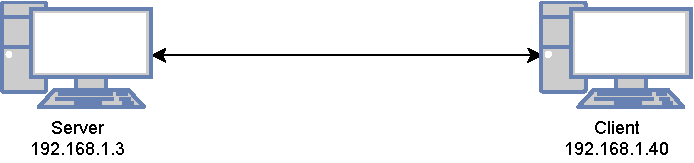
\includegraphics[width=0.8\textwidth]{img/__09__datagrams/dgram_test_env.pdf}
  \caption{Test environment}
  \label{fig:dgram_test_env}
\end{figure}
\subsection{Flow control}
As stated above DATAGRAM frames are not subject to flow control mechanism.
Thanks to this we can limit data that can be sent in a reliable way to allow for better unreliable communication.
\subsubsection{Tests}
This test illustrates DATAGRAMs behavior in case of reaching flow control limit on any of streams used in the connection.
Test environment was described in \ref{sec:test_env}.
Client opens two bidirectional streams while server sets their flow control limit to 1000B.
In each iteration client tries to send 10 reliable and 10 unreliable messages of size 800B each.
Figure \ref{fig:dgram_flow_control} presents this scenario.

\begin{figure}
  \centering
  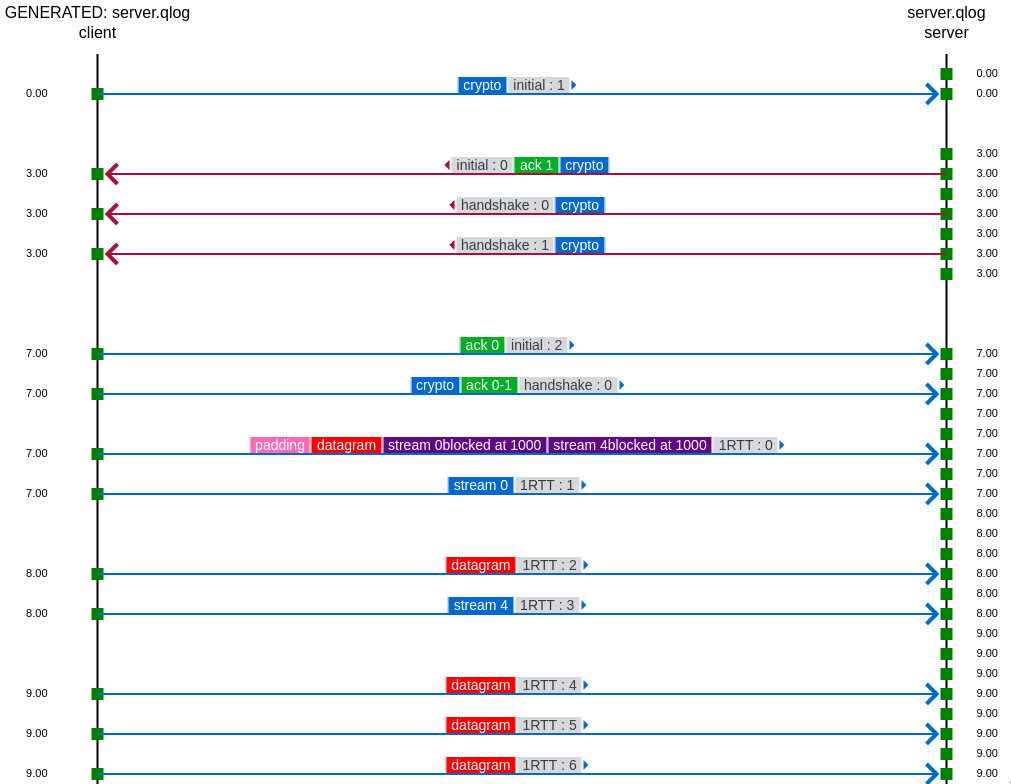
\includegraphics[width=\textwidth]{img/__09__datagrams/dgram_flow_control.png}
  \caption{DATAGRAM flow control test}
  \label{fig:dgram_flow_control}
\end{figure}

After establishing the connection client starts sending data.
He sends two 1-RTT packets with STREAM frames (packets 1 and 3) and reaches flow control limit.
However, he is still able to send packets with DATAGRAM frames (packets 4, 5, 6).

% \begin{figure}[h]
%   \centering
%   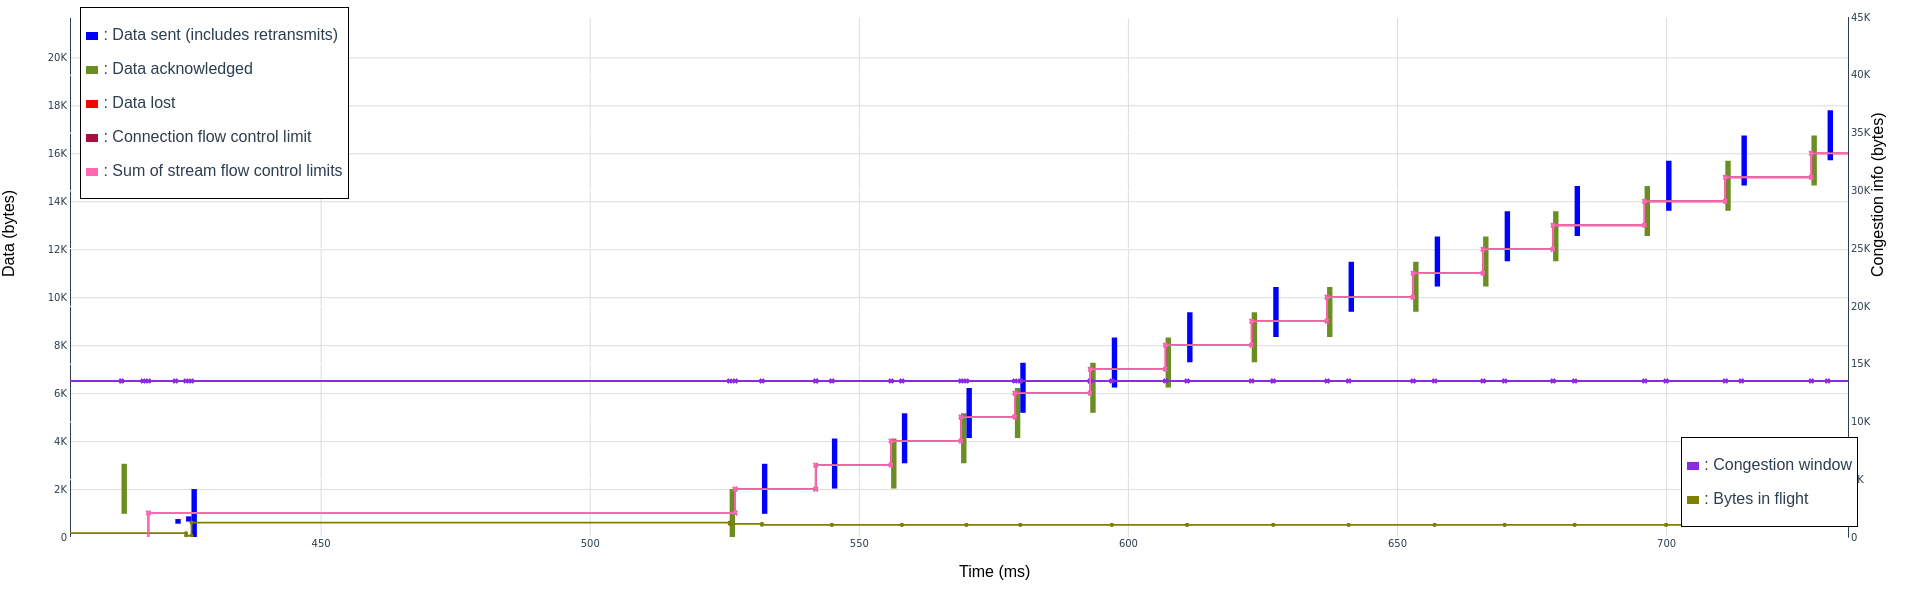
\includegraphics[width=\textwidth]{img/__09__datagrams/stream_flow_control_2.png}
%   \caption{DATAGRAM flow control test}
%   \label{fig:stream_flow_control2}
% \end{figure}

Figure \ref{fig:dgram_flow_control2} shows this behavior from different perspective.
\begin{figure}
  \centering
  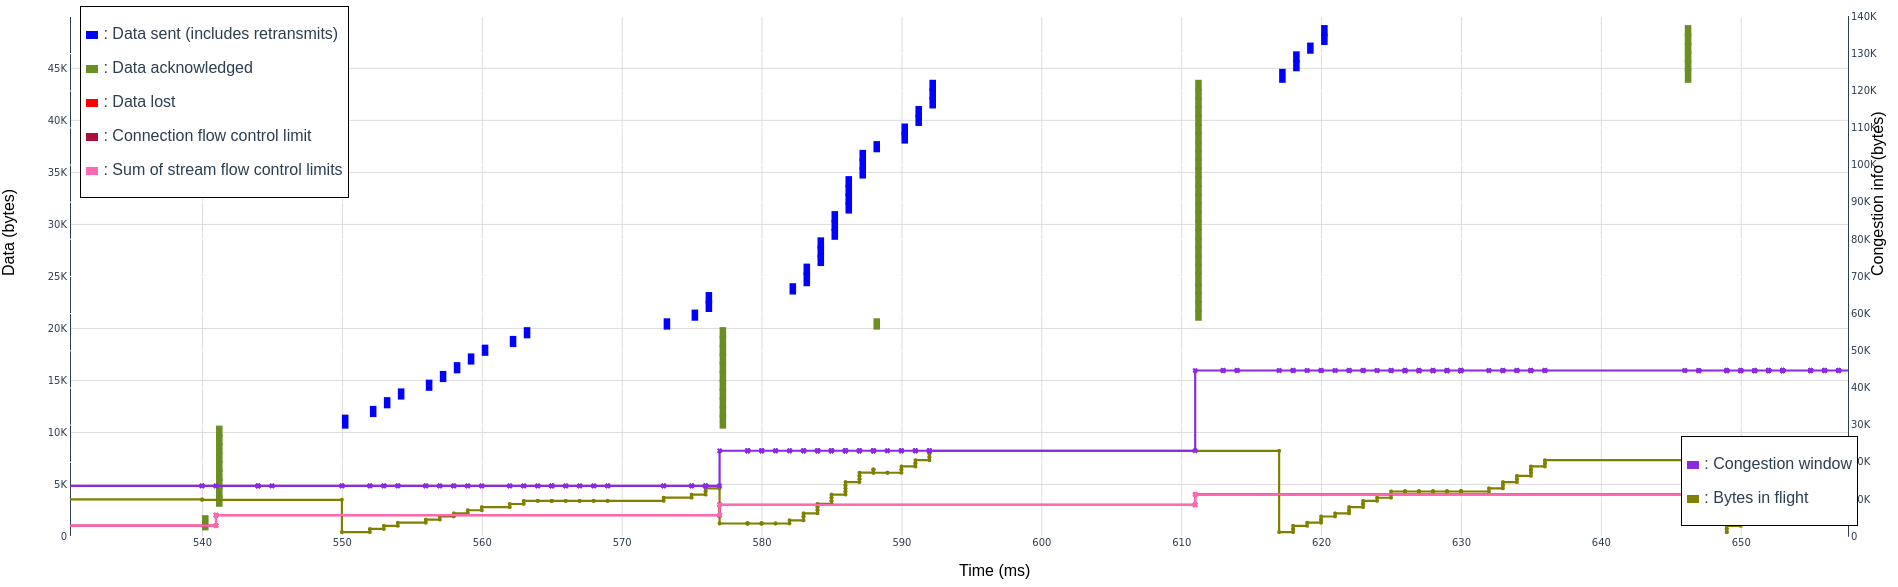
\includegraphics[width=\textwidth]{img/__09__datagrams/dgram_flow_control_2.png}
  \caption{DATAGRAM flow control test}
  \label{fig:dgram_flow_control2}
\end{figure}
Pink line indicates sum of stream flow control limit whereas blue bars represent data sent. 
We can see that despite the fact flow control limit is less than 5kB we send much more data -- over 45kB.

\subsection{Loss detection}
\label{sec:loss-detection}
From RFC 9002 (Section 6.1), a packet is declared lost if it meets all of the following conditions:
\begin{itemize}
    \item The packet is unacknowledged, in flight, and was sent prior to an acknowledged packet.
    \item The packet was sent kPacketThreshold packets before an acknowledged packet (Section 6.1.1), or it was sent long enough in the past (Section 6.1.2). \cite{rfc9002}
\end{itemize}

What is important is that to consider packet is lost there has to be some other packet that was sent later and has already been acknowledged.

\subsubsection{PTO}
A Probe Timeout (PTO) triggers the sending of one or two probe datagrams when ack-eliciting packets are not acknowledged within the expected period of time or the server may not have validated the client's address. A PTO enables a connection to recover from loss of tail packets or acknowledgments \cite{rfc9002} (RFC 9002, Section 6.2).

Expiration of PTO timer does not indicate the packet was lost.
It only provides one of the requirements necessary to consider the packet as lost -- the packet was sent prior to an acknowledged packet. PTO timer is reset each time a new ack-elicting packet was sent or received.

\subsubsection{Tests}
This test illustrates the impact of packet loss on communication with DATAGRAM frames.
Test environment was described in \ref{sec:test_env}.
Additionally, in some scenarios client machine had some packet loss set for all UDP datagrams which destination port was equal to 4433.
This was done using Linux TC software. 

The test consists of three scenarios.
In each scenario client was trying to send 1000 messages of 500B size each.
Server responsibility was to respond for each message by returning it back to the client.
After sending each message client was waiting for the response from the sever specified amount of time.
The summary is presented in table \ref{tab:dgram_packet_loss}.

\begin{table}
\centering
\resizebox{\columnwidth}{!}{%
\begin{tabular}{|c | c | c | c | c | c |} 
    \hline
    \multicolumn{2}{|c}{\makecell{0\% packet loss}} & \multicolumn{2}{|c}{\makecell{10\% packet loss}}  & \multicolumn{2}{|c|}{\makecell{30\% packet loss}} \\
    \hline
    \multicolumn{2}{|c}{client} & \multicolumn{2}{|c|}{client} & \multicolumn{2}{|c|}{client} \\
    \hline
    packets sent & packets lost & packets sent & packets lost & packets sent & packets lost \\  
    \hline
    1005 & 0 & 1007 & 89 & 1031 & 318 \\ 
    \hline
\end{tabular}%
}
\caption{\label{tab:dgram_packet_loss}Number of packets sent with and without packet loss for DATAGRAM frames.}
\end{table}

In the first scenario messages were sent via DATAGRAM frames without packet loss.
As a result client sent 1005 packets. None of them were lost.

In the second scenario messages were sent via DATAGRAM frames but packet loss was set to 10\%.
As a result client sent 1007 packets, 89 of which were lost. 
We can see that in this scenario client sent 2 packets more than in the first scenario.
This is because server sends its data as last and client need to acknowledge this data by sending additional packet with ACK frame but it is not important.

In the last scenario, messages were sent via DATAGRAM frames but packet loss was set to 30\%.
As a result client sent 1031 packets, 318 of which were lost.
This time we can observe that client sent ~20-30 packets more than in the first two scenarios.
It's because of PING frames that are being sent when PTO timer expires. 
Figure \ref{fig:dgram_ping_frames} illustrates this situation.
 
\begin{figure}
  \centering
  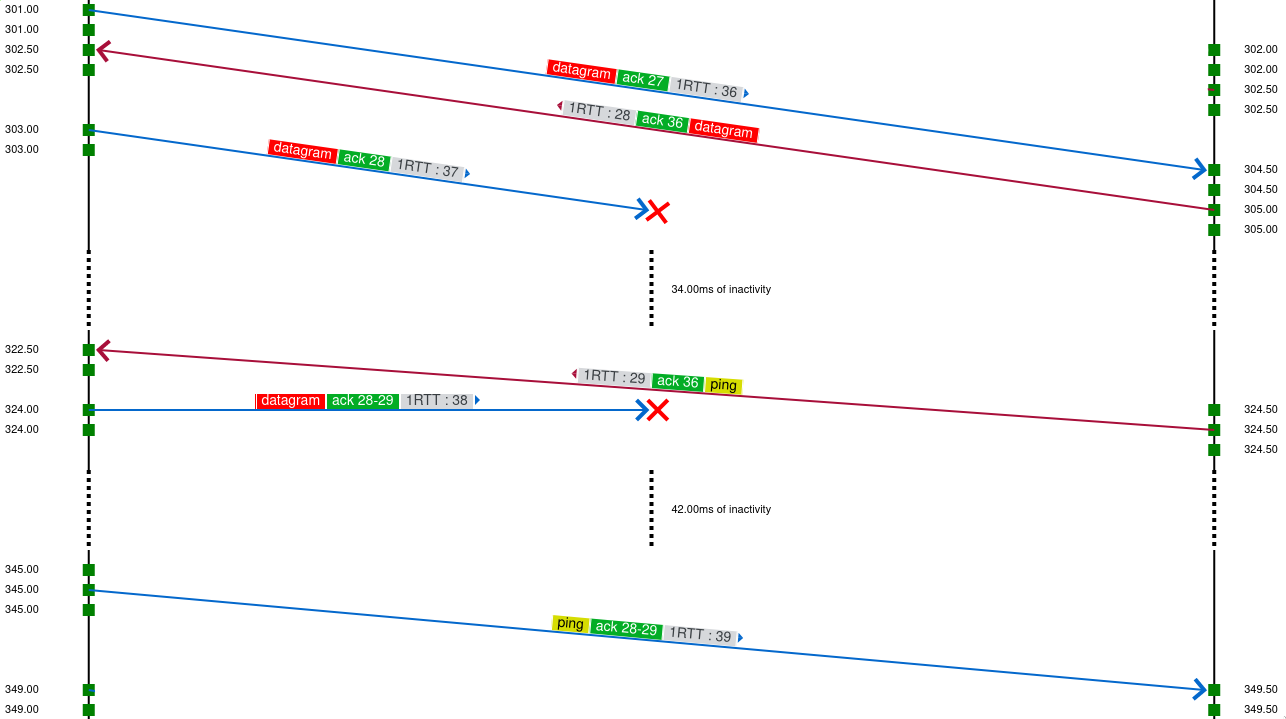
\includegraphics[width=\textwidth]{img/__09__datagrams/dgram_retransmission_ping.png}
  \caption{Sending PING frame after server or client inactivity. 
  Client messages are described by blue arrows. 
  Numbers on the left and right side indicate time in ms when given packet was sent or received.}
  \label{fig:dgram_ping_frames}
\end{figure}

Server in its 28th 1RTT packet sent datagram frame in response to client's earlier packet and set its PTO timer.
Client received server's packet, generated a response and set its own timer.
The response was lost so that server's PTO timer expired which resulted in 29th 1RTT packet from server to client with PING frame. 
After receiving it client generated a response, reset its PTO timer and sent the response but this time it was also lost.
After 21 ms client's PTO timer expired so client sent a new ack-elicting packet with PING frame.

    \clearpage
    \section{Conclusions}
\label{sec:conclusions}
QUIC is a new transport protocol that is intended to replace TCP\@.
Although it is general purpose transport protocol, in most cases it has been deployed in conjunction with HTTP/3 so far.
This document brings QUIC to a new domain called interactive communication.

In terms of interactive communication some of the crucial mechanisms are QUIC encryption process and DATAGRAM frames.
This document shows that none of them introduces a significant overhead to the connection bandwidth usage or transmission delay.
Current systems can take advantage of QUIC reducing their complexity and becoming easier to maintain and develop.
In this context ability to multiplex many logical channels, both reliable and unreliable in one physical connection seems to be invaluable.

However, additional experiments are needed to clearly state if QUIC is a better choice than existing protocols.
The most important area that requires further examination is congestion control.
Advanced and detailed test scenarios in appropriately complex global network are crucial for determining its behaviour.
Performing such experiments in a local configuration would not represent sufficiently real conditions.

    \clearpage
    \section{Video}
\label{sec:video}

\subsection{Architecture}
\label{subsec:architecture}

Figure~\ref{fig:video-app-architecture} illustrates architecture of video quic application.


\begin{figure}
    \centering
    \tikzstyle{rect}=[rectangle,minimum width=4cm,minimum height=1cm,draw=black]
    \scalebox{.75}{%
    \begin{tikzpicture}
        \node[label=below:{H264 video file}](file){
        \begin{tikzpicture}
            \draw (0,0) -- (0,1.2) -- (0.7,1.2) -- (0.7,0.8) -- (1,0.8) -- (1,0) -- cycle;
            \draw (0.7,1.2) -- (1,0.8);
            \foreach \y in {0.2,0.4,0.6}{
            \draw (0.2,\y) -- (0.8,\y);
            \draw (0.2,0.8) -- (0.6,0.8);
            \draw (0.2,1) -- (0.6,1);
            }
        \end{tikzpicture}
        };
        \node[rect,below=of file] (file-src) {File Source}
        edge [<-] node[align=center,right] {} (file);
        \node[rect,below=of file-src] (video-parser) {Video Parser}
        edge [<-] node[align=center,right] {} (file-src);
        \node[rect,below=of video-parser] (rtp-session-bin) {RTP Session Bin}
        edge [<-] node[align=center,right] {} (video-parser);
        \node[rect,below=of rtp-session-bin] (realtimer) {Realtimer}
        edge [<-] node[align=center,right] {} (rtp-session-bin);
        \node[rect,below=of realtimer] (quic-sink) {Quic Sink}
        edge [<-] node[align=center,right] {} (realtimer);
        \node[below=of quic-sink, label=center:Internet] (internet) {
\includegraphics{cisco_icons/cloud.eps}}
        edge [<-] node[align=center,right] {} (quic-sink);
        \node[rect,below=of internet] (quic-src) {Quic Source}
        edge [<-] node[align=center,right] {} (internet);
        \node[rect,below=of quic-src] (rtp-session-bin-2) {RTP Session Bin}
        edge [<-] node[align=center,right] {} (quic-src);
        \node[rect,below=of rtp-session-bin-2] (video-parser-2) {Video Parser}
        edge [<-] node[align=center,right] {} (rtp-session-bin-2);
        \node[rect,below=of video-parser-2] (video-decoder) {Video Decoder}
        edge [<-] node[align=center,right] {} (video-parser-2);
        \node[rect,below=of video-decoder] (sdl-player) {SDL player}
        edge [<-] node[align=center,right] {} (video-decoder);

        \node[rect,dashed,minimum width=12cm,fit=(file)(quic-sink)] (server-side) {};
        \node[rect,dashed,minimum width=12cm,fit=(quic-src)(sdl-player)] (client-side) {};
        \node[right] at (server-side.west) {\large server side};
        \node[right] at (client-side.west) {\large client side};
    \end{tikzpicture}%
    }
    \label{fig:video-app-architecture}
    \caption{Architecture of video quic application}
\end{figure}


    \clearpage

    \bibliographystyle{plain}
    \bibliography{bibliografia}

\end{document}
